\documentclass[11pt]{article}
\usepackage[T1]{fontenc}
\usepackage[utf8]{inputenc}
\usepackage{lmodern}
\usepackage[margin=1in]{geometry}
\usepackage{amsmath,amssymb,amsthm,mathtools}
\usepackage{microtype}
\usepackage{booktabs}
\def\DoNotLoadEpstopdf{}
\usepackage{tikz}
\usetikzlibrary{arrows.meta,positioning,calc,decorations.pathreplacing}
\usepackage[unicode,colorlinks=true,linkcolor=blue,citecolor=blue,urlcolor=blue]{hyperref}
\usepackage{bookmark}
\pdfinfoomitdate=1
\pdftrailerid{}
\pdfsuppressptexinfo=15
\newtheorem{theorem}{Theorem}[section]
\newtheorem{lemma}[theorem]{Lemma}
\newtheorem{proposition}[theorem]{Proposition}
\newtheorem{corollary}[theorem]{Corollary}
\theoremstyle{definition}
\newtheorem{definition}[theorem]{Definition}
\theoremstyle{remark}
\newtheorem{remark}[theorem]{Remark}
\newcommand{\R}{\mathbb R}
\newcommand{\T}{\mathbb T}
\newcommand{\E}{\mathbb E}
\newcommand{\Pbb}{\mathbb P}
\newcommand{\N}{\mathbb N}
\hypersetup{pdftitle={The dyadic case of the Erdos similarity conjecture},pdfauthor={OpenAI}}
\title{The dyadic case of the Erd\H{o}s similarity conjecture}
\author{OpenAI}
\date{September 25, 2026}
\begin{document}
\maketitle
\begin{abstract}
We construct a compact subset of the unit interval, of measure arbitrarily
close to one, that contains no affine copy of the dyadic sequence
$\{2^{-n}:n\ge1\}$. The conclusion holds for every translation and every
nonzero real dilation, of either sign, proving the dyadic case of the
Erd\H{o}s similarity conjecture.
\end{abstract}
\tableofcontents
\section{Introduction}\label{sec:introduction}

Let $m$ denote Lebesgue measure on $\R$. For a set $A\subseteq\R$, a
\emph{nontrivial affine copy} of $A$ is a set
\[
 x+sA=\{x+sa:a\in A\},\qquad x\in\R,\quad s\in\R\setminus\{0\}.
\]
The set $A$ is \emph{measure universal} if every Lebesgue-measurable subset
of $\R$ of positive measure contains such a copy. The Erd\H{o}s similarity
conjecture asserts that no infinite subset of $\R$ is measure universal;
the problem was posed by Erd\H{o}s in
\cite[Problem~4.33.7*]{Erdos1974Problems}.
Every nonempty finite pattern $F$ is measure universal. Indeed, if a measurable
set contains a subset $E_0$ of finite positive measure, translation
continuity in $L^1$ gives
$m(\bigcap_{a\in F}(E_0-sa))\to m(E_0)>0$ as $s\to0$.
A point in this intersection supplies an affine copy of $F$.
The difficulty therefore lies in keeping infinitely many points in the
same positive-measure set. We consider the single sequence
\[
 D=\{2^{-n}:n\in\N,\ n\ge1\}.
\]

\begin{theorem}\label{thm:main}
For every $\eta\in(0,1)$, there is a compact set $E_\eta\subseteq[0,1]$
with $m(E_\eta)>1-\eta$ such that
\[
 \text{for every }x\in\R\text{ and every }s\in\R\setminus\{0\},
 \quad x+sD\nsubseteq E_\eta.
\]
Equivalently, for every such $x,s$ there is an integer $n\ge1$ with
$x+s2^{-n}\notin E_\eta$.
\end{theorem}

Thus the dyadic sequence is not measure universal. The theorem concerns
one infinite pattern and all of its signed affine copies; the conjecture
for arbitrary infinite sets is not addressed. Compactness and the
near-full-measure conclusion follow directly from the open sets used in
the construction.

\subsection{Related results}

Classical results concern slowly decreasing sequences.
Falconer~\cite{Falconer1984} and Eigen~\cite{Eigen1985} proved
nonuniversality for positive sequences $a_n\downarrow0$ with
$a_{n+1}/a_n\to1$; see also the proof in
\cite[Corollary~1]{HumkeLaczkovich1998}.
Humke and Laczkovich give a finite hitting-set characterization and
further relative-gap criteria \cite[Theorems~1--2]{HumkeLaczkovich1998}.
Kolountzakis's finite-gap criterion uses arbitrarily large finite subsets
of a positive sequence: the minimum gaps, divided by their largest points,
must have negative logarithms growing sublinearly in the cardinalities
\cite[Theorem~3]{Kolountzakis1997}. Chleb\'ik gives a translation-invariant
formulation normalized by the diameter
\cite[Theorem~15]{Chlebik2015}. Dyadic subsets do not satisfy either
condition: for $n\ge2$ dyadic points $a_1>\cdots>a_n$, the minimum gap
is at most $a_{n-1}\le2^{-(n-2)}a_1$, whereas the diameter
$a_1-a_n$ is at least $a_1/2$. Either normalized minimum gap is therefore
at most $2^{-(n-3)}$.

Additive structure gives another family of results. Bourgain proved
that a sum of three infinite sets is nonuniversal
\cite{Bourgain1987}, and Kolountzakis treated sums of two copies of
certain sequences, including $D+D$ \cite[Section~3.4]{Kolountzakis1997}.
The distinction between the dyadic sequence and larger patterns is
important. Mora Cu\'ellar, Iosevich, Kulkarni, Rojas Aravena and Yavicoli
prove nonuniversality for the sum or difference of a nonconstant geometric
sequence tending to zero and an arbitrary infinite set
\cite[Theorem~2]{MoraCuellarEtAl2026Twofold}. Their Introduction explicitly
separates the single dyadic sequence from this two-fold sumset result.
Avoiding a larger pattern does not imply avoidance of a subset of that
pattern.

Iosevich, Kulkarni, Mora Cu\'ellar, Rojas Aravena and Yavicoli prove a
nonuniversality criterion for sets supporting a Rajchman probability
measure, that is, a probability measure whose Fourier transform tends to
zero at infinity \cite[Theorem~1.5]{IKMRY2026Rajchman}. A countable set
cannot support such a measure \cite[Proposition~4.1]{IKMRY2026Rajchman},
so that criterion does not apply to $D$. Their more general
uniform-density criterion on the circle
\cite[Proposition~3.2]{IKMRY2026Rajchman} also fails for
$D\cup\{0\}$: for every integer $k\ge1$, dilation by $2^k$ leaves its
image modulo one unchanged,
and that image stays a distance $1/4$ from $3/4$.

Other notions of size and other transformation classes also lead to
different questions. For certain sequences tending to zero, Cruz, Lai and
Pramanik obtain sets of Hausdorff dimension one avoiding affine copies of
the sequence together with its limit point; the avoiding sets in their
construction have Lebesgue measure zero
\cite[preprint, Corollary~1.2 and Proposition~4.4]{CruzLaiPramanik2023}.
In the other direction,
Feng, Lai and Xiong's bi-Lipschitz embedding theorem applies to the dyadic
sequence \cite[preprint, Theorem~1.1]{FengLaiXiong2024}. Such nonlinear embeddings
are compatible with the affine nonuniversality in Theorem~\ref{thm:main}.
A separate earlier preprint of Cruz, Lai and Pramanik claiming the full
similarity conjecture was withdrawn because of a gap in its
Proposition~3.3 \cite{CruzLaiPramanik2020Withdrawn}.

\subsection{The construction}

Our main step is to construct an open, $1$-periodic set of small density
that meets every $x+tD$ with $x\in\R$ and $t\in[1,2]$. The next section
states this intermediate result precisely. Dyadic rescaling and
reflection then produce a small open set meeting every signed affine
copy of $D$; its complement in $[0,1]$ is the desired compact set.
Periodic blocking sets and summable measure budgets also appear in
\cite[Lemma~3.1 and Proposition~3.2]{IKMRY2026Rajchman}; the finite construction below supplies
the required hitting property for $D$.

Random cell constructions, discretization of the dilation parameter at
a fixed center, and integration over centers occur in
Kolountzakis \cite[Section~3.2]{Kolountzakis1997},
Chleb\'ik \cite[Section~5]{Chlebik2015}, and
Kolountzakis--Papageorgiou
\cite[Section~3.1]{KolountzakisPapageorgiou2025}.
Exceptional centers are repaired by an open cover in Kolountzakis
\cite[Sections~2.2 and~3.2]{Kolountzakis1997}; Chleb\'ik also describes
adding the centers themselves when the pattern contains zero
\cite[Section~3, final remark]{Chlebik2015}.
We use the open-neighborhood form, since $0$ is a limit point of $D$
but is not in $D$.
An earlier attempt to extend the random-cell approach to the dyadic
sequence is described by Solymosi \cite[Section~3]{Solymosi2011Sparse};
that report does not claim a completed construction.
The argument below implements these principles with separated index
windows and a finite routing construction. All estimates needed for the
proof are supplied here.

To construct the periodic set, we first assign each point of the line to
one leaf of a finite ordered tree with $M$ children at each internal
node and $d$ levels. Independent fair binary tables, evaluated on
dyadic cells, determine the route. At each node, the first successful
test chooses a child; if all tests fail, the last child is chosen by
default. Each leaf carries a second table
whose entries select points with a small prescribed probability $p$.
This keeps the expected density small.

At a node, the default child is chosen only when all $M-1$ tested bits
vanish. Although this is rare for large $M$, taking the depth $d$
sufficiently large makes a default somewhere along the center's route
likely. At the first such node, all nondefault choices have been rejected
by the center. Carefully chosen dyadic translates preserve the route to
that node and its earlier rejections, but consult fresh entries at their
current-window resolution. Many nondefault children and many translates
then supply many potential hits.

Two features make those tests useful simultaneously for every normalized
scale. First, an interval of dyadic indices is assigned to each edge, in
the order in which the tree is traversed. Gaps between these intervals
preserve the earlier routing decisions for all but a small set of
centers. Second, each interval is long enough to control every cell
resolution in its child subtree. This bounds the number of different
local tests as the scale varies. We expose the tables in stages, proving
that the terminal entries used by these adaptively chosen routes are
distinct before multiplying their failure probabilities. A finite union
bound then controls all scales in $[1,2]$.

The resulting set may still miss copies centered in a small closed set.
An open neighborhood of those centers repairs every such copy, since
$x+t2^{-n}$ converges to $x$. This last step is what changes an estimate
on exceptional centers into a statement valid at every center.

The windows and their spatial stability are constructed in
Section~\ref{sec:windows}. Section~\ref{sec:routing} defines the random
set and proves the independent-trial estimate.
Section~\ref{sec:scales} handles the continuum of normalized scales and
removes the exceptional centers. Section~\ref{sec:global} completes the
signed-scale deduction of Theorem~\ref{thm:main}.

\section{The periodic hitting problem}\label{sec:periodic}

For a measurable $1$-periodic set $A\subseteq\R$, write
\[
 \rho(A)=m(A\cap[0,1])
\]
for its density in one period. We will sometimes identify such a set
with its image in the circle $\T=\R/\mathbb Z$, equipped with normalized
Lebesgue measure. This identification preserves the density. Open or
closed subsets of the circle lift to open or closed periodic subsets of
$\R$.

\begin{lemma}[Periodic hitting sets]\label{lem:periodic}
For every $p\in(0,1)$, there exists an open $1$-periodic set $H\subseteq\R$
such that $\rho(H)\le6p$ and
\[
 \forall x\in\R\ \forall t\in[1,2]\ \exists n\in\mathbb Z_{\ge1}:
 \qquad x+t2^{-n}\in H.
\]
\end{lemma}

The same set $H$ works for every center and every scale in the displayed
interval. The witness $n$ may depend on both. In
Section~\ref{sec:global}, we apply the lemma with a summable sequence of
parameters, rescale the resulting periodic sets by powers of two, and
include their reflections. This handles every nonzero real scale while
keeping the total measure removed from $[0,1]$ small.

For the proof of Lemma~\ref{lem:periodic}, fix $p\in(0,1)$. We construct
a random periodic set $B$ with expected density $p$, together with a
finite set $\mathcal N$ of positive integer indices. Outside a
deterministic set of centers of density less than $p$, the probability
that some $t\in[1,2]$ avoids $B$ at all indices in $\mathcal N$ will be
at most $2p$. We then enlarge $B$ to an open set, bound the expected
measure of its exceptional centers, and cover those centers by a small
open set. The last step uses further indices in the dyadic tail;
$\mathcal N$ need not provide the hits at the repaired centers.

\section{Separated index windows}\label{sec:windows}

We first assign a finite block of dyadic indices to every edge of an
ordered tree.  Gaps between the blocks will let small translations
preserve earlier grid cells.  Each block will also be long enough to
control all resolutions needed below its child.  These two properties
will serve different purposes in the random construction.

\subsection{The tree and the window lengths}

Fix $p\in(0,1)$.  Choose integers $M\ge2$ and $d\ge1$ such that
\begin{equation}
 \frac{p(M-1)}2\ge10,
 \qquad
 (1-2^{1-M})^d<p.
 \label{eq:tree-parameters}
\end{equation}
Such choices can be made in this order: the first inequality holds for
large enough $M$, after which $0<1-2^{1-M}<1$ permits the second choice.
Let $\mathcal T$ be the complete ordered tree of height $d$ in which each
internal vertex has $M$ children.  Its root has height $d$, its leaves
have height $0$, and the children of an internal vertex $P$ are
$P_1,\ldots,P_M$.  Write $e=(P,i)$ for the edge from $P$ to $P_i$.
The finite total number of edges is
\[
 K=\sum_{\ell=1}^d M^\ell.
\]
List the edges in the following preorder: for each vertex $P$, list
$(P,1)$ and all edges below $P_1$, then $(P,2)$ and all edges below
$P_2$, and so on.  Thus an edge together with all edges below its child
forms one consecutive block in the list.

Choose an integer $g\ge1$ such that
\begin{equation}
 K2^{2-g}<p.
 \label{eq:gap-budget}
\end{equation}
This choice depends only on the already fixed tree.  We will leave $g$
unused indices between consecutive windows.

The $M-1$ nondefault child windows of a node, each of length $r$, will
together supply $(M-1)r$ random tests at a fixed scale $t\in[1,2]$.
The exponential factor in the next inequality will bound
the probability that all these tests fail. The preceding factor will
bound the size of a finite list of scale values that represents every
possible collection of local grid keys as $t$ varies. Making their
product small will control all normalized scales by a finite union
bound; Sections~\ref{sec:routing} and~\ref{sec:scales} prove these two
bounds.

Choose an integer $r_*\ge1$ such that, for every integer
$r\ge r_*$,
\begin{equation}
 20Mr(1+2^{2r+2})
       \exp\!\left(-\frac{p(M-1)}2r\right)<p.
 \label{eq:entropy-budget}
\end{equation}
For completeness, the left side is at most $100M e^{-7r}$ when $r\ge1$:
use \eqref{eq:tree-parameters},
$1+2^{2r+2}\le5e^{2r}$, and $r\le e^r$.
Hence any integer $r_*>\log(100M/p)/7$ works simultaneously for all
larger $r$.  The uniformity will allow us to enlarge windows as needed.

We assign a window length $r_h$ to edges whose parent has height $h$.
At the same time we compute the span $\sigma_h$ of all windows in a
subtree of height $h$, including the gaps between them.  Starting with
$\sigma_0=0$, define successively for $h=1,\ldots,d$
\begin{equation}
 \begin{split}
 r_h&=\max\{r_*,g+\sigma_{h-1}\},\\
 \sigma_h&=
 \begin{cases}
 Mr_1+(M-1)g,&h=1,\\
 M(r_h+g+\sigma_{h-1})+(M-1)g,&h\ge2.
 \end{cases}
 \end{split}
 \label{eq:window-recursion}
\end{equation}
This is a finite bottom-up recursion: $r_h$ depends only on lengths
already chosen below height $h$.  In particular, the choice of $g$ did
not depend on the sizes of these lengths.

Now place the actual integer windows in the edge preorder, starting at
$3$.  An edge $e$ from height $h$ receives
$W_e=\{a_e,\ldots,b_e\}$ with $b_e=a_e+r_h-1$; if $f$ immediately
precedes $e$, set $a_e=b_f+g+1$.  Put
\[
 \mathcal N=\bigcup_{e\in\mathcal T}W_e,
\]
where the union is over the edges of the tree.  The span interpretation
of \eqref{eq:window-recursion} follows by induction.  At height $1$
there are $M$ windows and $M-1$ gaps.  At height $h\ge2$, each child
block consists of an incoming window of length $r_h$, one gap, and a
subtree block of span $\sigma_{h-1}$; there are another $M-1$ gaps
between these child blocks.

For an edge $e=(P,i)$, let $b_e^*$ be the largest window endpoint among
$e$ and all edges below $P_i$.  If $P$ has height $h=1$, this block
consists only of $e$, and its span is $r_1$.  If $h\ge2$, its span is
$r_h+g+\sigma_{h-1}$.  Therefore in both cases
\begin{equation}
 b_e^*-a_e+1\le r_h+g+\sigma_{h-1}\le2r_h.
 \label{eq:padding}
\end{equation}
In particular, \eqref{eq:entropy-budget} applies to every length $r_h$,
while \eqref{eq:padding} bounds a whole child block in terms of its
incoming window.  All edges, including those with child index $M$,
receive windows under this construction.

The padding bound has a specific purpose: the range of window indices
from $a_e$ through $b_e^*$ in a child block is controlled by the length
of its incoming window. The gaps have a different role, established
next: for most centers, translations indexed by a later window preserve
the earlier cells used in the routing decisions. These
are the two deterministic inputs to the routing and scale-counting
arguments.

\begin{figure}[htbp]
\centering
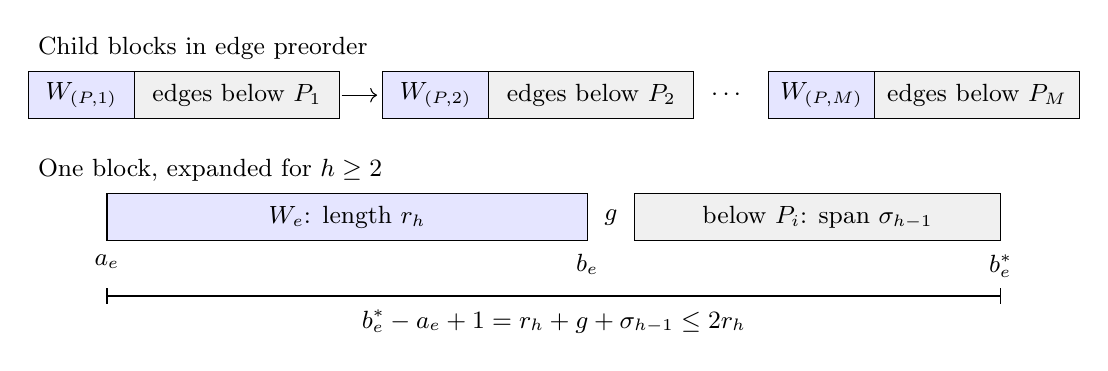
\begin{tikzpicture}[x=1cm,y=1cm,font=\small]
  \node[anchor=west] at (0,2.5) {Child blocks in edge preorder};
  \foreach \start/\index in {0/1,4.5/2,9.4/M}{
    \fill[blue!10] (\start,1.6) rectangle (\start+1.35,2.2);
    \fill[gray!12] (\start+1.35,1.6) rectangle (\start+3.95,2.2);
    \draw (\start,1.6) rectangle (\start+3.95,2.2);
    \draw (\start+1.35,1.6)--(\start+1.35,2.2);
    \node at (\start+.675,1.9) {$W_{(P,\index)}$};
    \node at (\start+2.65,1.9) {edges below $P_{\index}$};
  }
  \draw[->] (3.98,1.9)--(4.43,1.9);
  \node at (8.89,1.9) {$\cdots$};
  \node[anchor=west] at (0,.95) {One block, expanded for $h\ge2$};
  \fill[blue!10] (1,.05) rectangle (7.1,.65);
  \fill[gray!12] (7.7,.05) rectangle (12.35,.65);
  \draw (1,.05) rectangle (7.1,.65);
  \draw (7.7,.05) rectangle (12.35,.65);
  \node at (4.05,.35) {$W_e$: length $r_h$};
  \node at (7.4,.35) {$g$};
  \node at (10.025,.35) {below $P_i$: span $\sigma_{h-1}$};
  \node[anchor=north] at (1,0) {$a_e$};
  \node[anchor=north] at (7.1,0) {$b_e$};
  \node[anchor=north] at (12.35,0) {$b_e^*$};
  \draw (1,-.65)--(12.35,-.65);
  \draw (1,-.55)--(1,-.75);
  \draw (12.35,-.55)--(12.35,-.75);
  \node[anchor=north] at (6.675,-.7)
    {$b_e^*-a_e+1=r_h+g+\sigma_{h-1}\le2r_h$};
\end{tikzpicture}
\caption{Each edge window precedes the windows below its child, and
the child blocks are listed in order.  The lower diagram includes the
gap before a nonempty child subtree.  An edge into a leaf has no
following subtree or internal gap.  Lengths are schematic.}
\label{fig:windows}
\end{figure}


\subsection{Earlier grid cells remain unchanged}

For every nonnegative integer $b$, define the periodic cell key
\begin{equation}
 J_b(z)=\left\lfloor2^{b+2}\{z\}\right\rfloor,
 \qquad \{z\}=z-\lfloor z\rfloor.
 \label{eq:grid-key}
\end{equation}
Its boundaries on the real line form the lattice
$\Gamma_b=2^{-(b+2)}\mathbb Z$.  In particular, every integer is a
boundary.  Cells are half-open on the right, so a boundary belongs to
the cell starting there.  The grids are nested: for $B\ge b$,
\begin{equation}
 J_b(z)=\left\lfloor\frac{J_B(z)}{2^{B-b}}\right\rfloor.
 \label{eq:grid-nesting}
\end{equation}
This follows by writing $2^{B+2}\{z\}=J_B(z)+\varepsilon$ with
$0\le\varepsilon<1$ and dividing by the integer $2^{B-b}$.

We seek centers for which translations indexed by one window preserve
every earlier grid key.  For a noninitial window $W_e$, let $b'$ be the
endpoint of the immediately preceding window, and put
$\delta_e=2^{1-a_e}$.  Call $x$ \emph{stable} if, for every such window,
\begin{equation}
 (x,x+\delta_e]\cap\Gamma_{b'}=\varnothing.
 \label{eq:stable-definition}
\end{equation}
Let $G$ denote the set of stable centers.  The intervals in
\eqref{eq:stable-definition} are taken on the real line, so crossings
of an integer are included without a separate convention on the circle.

\begin{lemma}\label{lem:stable}
The set $G$ is measurable and $1$-periodic, and $\rho(G^c)<p$.
For every $x\in G$, every window $W_e$, every $n\in W_e$, every
$t\in[1,2]$, and every window $W_f$ earlier than $W_e$,
\begin{equation}
 J_{b_f}(x+t2^{-n})=J_{b_f}(x).
 \label{eq:stable-keys}
\end{equation}
These assertions include centers lying on grid boundaries.
\end{lemma}

\begin{proof}
For a fixed noninitial window, the centers violating
\eqref{eq:stable-definition} are exactly
\[
 E_e=\bigcup_{\beta\in\Gamma_{b'}}[\beta-\delta_e,\beta),
\]
because $\beta\in(x,x+\delta_e]$ if and only if
$\beta-\delta_e\le x<\beta$.  This is a measurable periodic set.
Since $a_e=b'+g+1$,
\[
 2^{b'+2}\delta_e=2^{2-g}<p/K<1.
\]
Thus these intervals have disjoint interiors modulo one.  There are
$2^{b'+2}$ of them per period, each of length $\delta_e$, and hence
$\rho(E_e)=2^{2-g}$.  The complement of $G$ is the union of these sets
over the $K-1$ noninitial windows.  Consequently
\[
 \rho(G^c)\le(K-1)2^{2-g}<p.
\]
This also proves measurability and periodicity of $G$.

Now fix the data in \eqref{eq:stable-keys}.  If $W_e$ is the first
window, there is no earlier $W_f$.  Otherwise
$0<t2^{-n}\le2^{1-a_e}=\delta_e$, so stability implies that the
interval $(x,x+t2^{-n}]$ contains no boundary of $\Gamma_{b'}$.
Both endpoints therefore have the same $J_{b'}$ key.  This remains true
when $x$ itself is a boundary, since it belongs to the cell on its
right; landing on a boundary at a positive displacement has been
excluded.  An integer cannot lie in this interval either, so passing
to periodic keys introduces no additional case.  Finally, every earlier
window satisfies $b_f\le b'$, and \eqref{eq:grid-nesting} gives
\eqref{eq:stable-keys}.
\end{proof}

The tree, all windows, and $G$ are now fixed before any random choices.
The key agreement concerns earlier windows only.  This is the property
that will preserve the required earlier decisions while allowing tests
at the current window's finer resolution.

\section{Random routing and independent tests}
\label{sec:routing}

We now use the windows from the preceding section to construct a random
periodic set \(B\) of expected density \(p\).
Selectors send each spatial point to one leaf of the tree, where an
independent terminal entry decides membership in \(B\).
For a stable center, the first default choice on its path will provide
several child windows in which to test nearby points.

\subsection{The tables and the selected set}

For each edge \(e=(P,i)\) with \(i<M\), let
\[
 S_e:\{0,\ldots,2^{b_e+2}-1\}\longrightarrow\{0,1\}
\]
be a random table whose entries are independent Bernoulli variables
with parameter \(1/2\).
There is no selector table for the default edge \((P,M)\).
For a leaf \(L\), let \(b(L)\) be the endpoint of the window assigned
to its unique incoming edge, and let
\[
 T_L:\{0,\ldots,2^{b(L)+2}-1\}\longrightarrow\{0,1\}
\]
be a random table whose entries are independent Bernoulli variables
with parameter \(p\).
All entries of all selector and terminal tables are mutually
independent.  The tree and every table are finite, so these variables
define a finite product probability space \(\Omega\).  We write
\(\mathbb P\) and \(\mathbb E\) for its probability and expectation.

Given the tables and a point \(z\in\mathbb R\), start at the root.
At an internal node \(P\), choose the first child \(P_i\), \(i<M\),
for which
\[
 S_{(P,i)}\bigl(J_{b_{(P,i)}}(z)\bigr)=1.
\]
If all \(M-1\) values are zero, choose the default child \(P_M\).
Continue until reaching a leaf, denoted by \(L(z)\), and define
\begin{equation}
 \label{eq:random-set}
 B=\left\{z\in\mathbb R:
 T_{L(z)}\bigl(J_{b(L(z))}(z)\bigr)=1\right\}.
\end{equation}
The table rules use only periodic keys.  Since all grids in the
construction are nested, membership in \(B\) is constant on each cell
of the finest grid used.  Thus every realization of \(B\) is a
\(1\)-periodic measurable set, consisting of finitely many half-open
cells per period.

Let \(\mathcal S\) be the sigma-field generated by every entry of every
selector table.  For fixed \(z\), conditioning on \(\mathcal S\) fixes
\(L(z)\) and the key of its terminal entry.  That entry still has
probability \(p\) of being one, since terminal tables are independent
of all selectors.  Hence
\[
 \mathbb P(z\in B\mid\mathcal S)=p.
\]
Integrating over one period and interchanging the integral with the
finite weighted sum over \(\Omega\) gives
\begin{equation}
 \label{eq:mean-density}
 \mathbb E\rho(B)=\int_0^1\mathbb P(z\in B)\,dz=p.
\end{equation}

\subsection{Conditioning at a center}

For a fixed center \(x\in\mathbb R\), expose one entry from every
selector table, including those in subtrees not visited by its path.
The resulting sigma-field is
\begin{equation}
 \label{eq:center-exposure}
 \mathcal F_x
 =
 \sigma\left(
 S_e\bigl(J_{b_e}(x)\bigr):
 e=(P,i),\ i<M
 \right)
 \subseteq\mathcal S.
\end{equation}
An atom \(\xi\) of \(\mathcal F_x\) means the event specifying all
these exposed values; we write \(\mathbb P(\,\cdot\mid\xi)\) for
conditioning on that event.
Every such atom has positive probability.
The exposed addresses \((e,J_{b_e}(x))\) are deterministic once
\(x\) is fixed, with the table name \(e\) included in the address.
Consequently, on each atom, all remaining selector entries retain
their independent fair law, and all terminal entries retain their
independent Bernoulli-\(p\) law.

The exposed values determine the full path of \(x\).
When that path chooses a default child, let \(U\) denote its first
internal node at which this happens.  Thus the existence and identity
of \(U\) are determined by \(\mathcal F_x\).
The next estimate concerns the original product law, before an atom
of \(\mathcal F_x\) is fixed.

\begin{lemma}[A default choice on the center path]
 \label{lem:first-default}
For every fixed \(x\in\mathbb R\),
\[
 \mathbb P\bigl(\text{the path of \(x\) never chooses child \(M\)}\bigr)
 =
 (1-2^{1-M})^d<p.
\]
\end{lemma}

\begin{proof}
At any internal node, the default child is chosen exactly when its
\(M-1\) selector entries at \(x\) are all zero.  This has probability
\(2^{-(M-1)}=2^{1-M}\).

To compute the probability along the path, reveal the entries at an
internal node only when the path first reaches it.  The decisions
leading to that node use tables at its strict ancestors.  Its own
tables are distinct from all of those tables and have not yet been
revealed, so their entries at \(x\) remain independent fair bits,
conditional on the preceding path history.
At each of the \(d\) internal-node decisions, the conditional
probability of a non-default choice is therefore \(1-2^{1-M}\).
Iterating this conditional probability gives
\((1-2^{1-M})^d\).  The strict inequality is the choice of \(d\) in
\eqref{eq:tree-parameters}.
\end{proof}

\subsection{Routing trials through the first default}

Fix henceforth a stable center \(x\in G\), and condition on an atom
\(\xi\) of \(\mathcal F_x\) for which \(U\) exists.
The node \(U\) is fixed under this conditioning.  Let \(h\) be its
height, and write
\[
 r=r_h,\qquad e_i=(U,i),\qquad b_i^*=b_{e_i}^*
 \quad(1\le i<M),\qquad y_n(t)=x+t2^{-n}.
\]
At \(U\), all the exposed non-default selector values are zero.

For \(i<M\) and \(z\in\mathbb R\), let \(L_i(z)\) be the leaf obtained
by applying the same path rule starting at the child \(U_i\).
If \(U_i\) is already a leaf, set \(L_i(z)=U_i\).
Define the local predicate
\begin{equation}
 \label{eq:local-predicate}
 Q_i(z)=
 S_{e_i}\bigl(J_{b_{e_i}}(z)\bigr)\,
 T_{L_i(z)}\bigl(J_{b(L_i(z))}(z)\bigr).
\end{equation}
The function \(Q_i\) takes values in \(\{0,1\}\) and consults only
the selector on \(e_i\) and tables in the subtree rooted at \(U_i\).
It provides a sufficient condition for membership in \(B\) at the
points indexed by \(W_{e_i}\).

\begin{lemma}[Preservation of the route]
 \label{lem:routing}
For every outcome in \(\xi\), every \(i<M\), every \(n\in W_{e_i}\),
and every \(t\in[1,2]\), the actual root path of \(y_n(t)\) reaches
\(U\) and rejects children \(1,\ldots,i-1\) there.
In particular,
\begin{equation}
 \label{eq:local-hit}
 Q_i(y_n(t))=1
 \quad\Longrightarrow\quad y_n(t)\in B.
\end{equation}
\end{lemma}

\begin{proof}
Consider a strict ancestor \(P\) of \(U\), and let \(P_a\) be its
child on the path of \(x\) to \(U\).
Since \(U\) is the first default node, \(a<M\).
The decision at \(P\) uses precisely the zero values of the selectors
\(1,\ldots,a-1\) and the value one of selector \(a\).
Each of the edges \((P,j)\), \(j\le a\), precedes every edge in the
subtree of \(P_a\) in the prescribed preorder.
Their windows therefore precede \(W_{e_i}\).
By the stable-key identity \eqref{eq:stable-keys},
each of these selector evaluations at \(y_n(t)\) agrees with its
evaluation at \(x\).
Induction from the root along the ancestor chain shows that
\(y_n(t)\) makes the same choices and reaches \(U\).
Later sibling selectors at an ancestor are not needed to make its
choice.

For every \(j<i\), the edge \((U,j)\) also precedes \(e_i\).
Its selector value at \(x\) is zero, because \(x\) takes the default
child at \(U\).
Another application of \eqref{eq:stable-keys} makes the corresponding
value at \(y_n(t)\) zero.
Thus the actual path rejects children \(1,\ldots,i-1\) at \(U\).

If \(Q_i(y_n(t))=1\), the selector on \(e_i\) is one, so the actual
path chooses child \(i\) at \(U\).
Its continuation is exactly the rule defining \(L_i(y_n(t))\),
and the terminal entry in \eqref{eq:local-predicate} is one.
The membership rule \eqref{eq:random-set} now gives \(y_n(t)\in B\).
Figure~\ref{fig:routing} records this common-prefix and branching argument.
All equalities used here hold for every completion of the unexposed
tables and every \(t\in[1,2]\), as required.
\end{proof}


\begin{figure}[!htb]
\centering
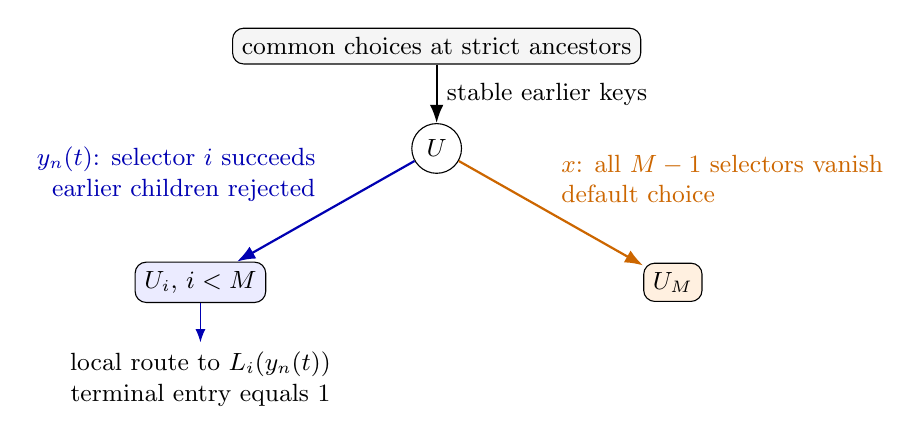
\begin{tikzpicture}[x=1cm,y=1cm,font=\small,>=Latex]
 \node[draw,rounded corners,fill=gray!8,minimum width=4.3cm] (prefix) at (0,3.15)
   {common choices at strict ancestors};
 \node[draw,circle,inner sep=3pt] (u) at (0,1.85) {$U$};
 \draw[->,thick] (prefix)--node[right] {stable earlier keys}(u);
 \node[draw,rounded corners,fill=blue!8] (childi) at (-3,.15) {$U_i$, $i<M$};
 \node[draw,rounded corners,fill=orange!12] (childm) at (3,.15) {$U_M$};
 \draw[->,thick,blue!70!black] (u)--node[above left,align=right]
   {$y_n(t)$: selector $i$ succeeds\\earlier children rejected}(childi);
 \draw[->,thick,orange!80!black] (u)--node[above right,align=left]
   {$x$: all $M-1$ selectors vanish\\default choice}(childm);
 \node[align=center,below=5mm of childi] (terminal)
   {local route to $L_i(y_n(t))$\\terminal entry equals $1$};
 \draw[->,blue!70!black] (childi)--(terminal);
\end{tikzpicture}
\caption{Route preservation for $x\in G$, $n\in W_{(U,i)}$ and
$t\in[1,2]$, conditional on $Q_i(y_n(t))=1$.
The center $x$ and its translate
$y_n(t)$ make the same required choices above the first default node $U$.
At $U$, the center takes child $M$, while the translate rejects the earlier
children and takes child $i$. The local terminal success then places
$y_n(t)$ in $B$. The diagram is conditional on the successful local
predicate; it does not assume independence of the chosen leaves.}
\label{fig:routing}
\end{figure}


\subsection{Independent terminal tests}

We now estimate the probability that all the local tests fail at one
fixed scale.  The selected leaves may depend on the selectors.  To keep
that dependence explicit, we first expose all selectors, identify the
terminal entries being read, and then average over the selectors.

\begin{lemma}[The fixed-scale estimate]
\label{lem:fixed-scale}
Fix a stable center \(x\) and an atom \(\xi\) of the center-exposure
sigma-field \(\mathcal F_x\) in \eqref{eq:center-exposure}, on
which the first default node \(U\) exists.  Let \(h\) be its height,
put \(r=r_h\), and use the local predicates \(Q_i\) for
\(e_i=(U,i)\), \(1\le i<M\), defined in \eqref{eq:local-predicate}, with \(y_n(t)=x+t2^{-n}\). For every fixed
\(t\in[1,2]\),
\begin{equation}
 \Pbb\left(
 Q_i(y_n(t))=0
 \text{ for all }1\le i<M,\ n\in W_{e_i}
 \,\middle|\,\xi
 \right)
 =(1-p/2)^{(M-1)r}.
 \label{eq:fixed-scale-miss}
\end{equation}
\end{lemma}

\begin{proof}
On the fixed atom \(\xi\), the node \(U\), the windows \(W_{e_i}\),
and the set of pairs
\[
 \mathcal I=\{(i,n):1\le i<M,\ n\in W_{e_i}\}
\]
are fixed.  Its cardinality is \((M-1)r\).  For these pairs define
\[
 A_{i,n}=S_{e_i}\bigl(J_{b_{e_i}}(y_n(t))\bigr).
\]
We first check that these are distinct selector entries, none of which
was exposed at \(x\).

Fix \(i\), and abbreviate \(a=a_{e_i}\) and \(b=b_{e_i}\).
For \(n<n'\) in this window,
\[
 y_n(t)-y_{n'}(t)
 =t\,2^{-n'}(2^{n'-n}-1)\ge 2^{-b}.
\]
Also \(y_n(t)-x=t2^{-n}\ge2^{-b}\).
All these points lie in \([x,x+2^{1-a}]\), an interval of length
at most \(1/4\), since \(a\ge3\).
Thus the circular distance between any two of them equals their
ordinary distance and is at least \(2^{-b}\).
Two points in the same half-open \(J_b\)-cell have circular distance
less than \(2^{-(b+2)}\).  Consequently the keys of
\(x\) and all \(y_n(t)\), \(n\in W_{e_i}\), are pairwise distinct.
This argument also covers a crossing of an integer and points on cell
boundaries.

For different \(i\), the selector tables themselves differ.
The variables \(A_{i,n}\) therefore read distinct coordinates outside
the entire exposed coordinate set defining \(\mathcal F_x\).
Conditional on \(\xi\), they remain independent fair bits.

Next condition on the sigma-algebra \(\mathcal S\) of all selectors.
For each pair, its selected local leaf
\[
 L_{i,n}=L_i(y_n(t))
\]
and its terminal address
\[
 \kappa_{i,n}=
 \bigl(L_{i,n},J_{b(L_{i,n})}(y_n(t))\bigr)
\]
are now fixed.  We claim that these addresses are distinct for all
pairs in \(\mathcal I\).
If the child indices differ, the leaves lie in disjoint child subtrees
of \(U\), so their terminal tables differ.
If the child indices agree but the leaves differ, their tables again
differ.  It remains to consider two different indices \(n,n'\) that
select the same leaf \(L\) below one child \(U_i\).

For every leaf below \(U_i\), its terminal resolution satisfies
\(b(L)\ge b_{e_i}\).  If \(U_i\) is a leaf, then \(b(L)=b_{e_i}\).
Otherwise the last edge into \(L\) occurs after \(e_i\) in the preorder,
so its window endpoint is larger.
By the nested-key identity~\eqref{eq:grid-nesting}, different keys at
resolution \(b_{e_i}\) remain different at resolution \(b(L)\),
including at grid boundaries.
The preceding separation of \(y_n(t)\) and \(y_{n'}(t)\) proves
\(\kappa_{i,n}\ne\kappa_{i,n'}\).
This proves the claim, even for pairs with \(A_{i,n}=0\).

The terminal tables are independent of \(\mathcal S\).
For each realization of all selectors, the addresses just identified
are fixed distinct coordinates of those tables.  The corresponding
terminal bits
\[
 V_{i,n}=
 T_{L_{i,n}}\bigl(J_{b(L_{i,n})}(y_n(t))\bigr)
\]
therefore have the product Bernoulli \(p\) law conditional on
\(\mathcal S\).  Since \(Q_i(y_n(t))=A_{i,n}V_{i,n}\),
only the pairs with \(A_{i,n}=1\) require a terminal bit to vanish.
On \(\xi\) we obtain
\[
 \Pbb\left(
 Q_i(y_n(t))=0\text{ for all }(i,n)\in\mathcal I
 \,\middle|\,\mathcal S
 \right)
 =(1-p)^{\sum_{(i,n)\in\mathcal I}A_{i,n}}.
\]
The empty-success case has exponent zero and probability one.

Finally, \(\mathcal F_x\subset\mathcal S\), so conditional expectation
and the independent fair law of the \(A_{i,n}\) on \(\xi\) give
\begin{align*}
 &\Pbb\left(
 Q_i(y_n(t))=0\text{ for all }(i,n)\in\mathcal I
 \,\middle|\,\xi
 \right)\\
 &\qquad=
 \E\left[(1-p)^{\sum_{(i,n)\in\mathcal I}A_{i,n}}
          \,\middle|\,\xi\right]\\
 &\qquad=
 \prod_{(i,n)\in\mathcal I}
 \left(\frac12+\frac12(1-p)\right)
 =(1-p/2)^{(M-1)r}.
\end{align*}
\end{proof}

The estimate applies separately to each scale fixed on the exposure
atom.  In the next step, the grid geometry will supply finitely many
such scales, allowing a union bound over all \(t\in[1,2]\).

\section{All normalized scales and all centers}
\label{sec:scales}

The preceding estimate concerns a fixed scale.  To control every
$t\in[1,2]$, we track the local predicates $Q_i$ on the grids of their
own child subtrees.  The padding of each window bounds the number of
changes in these predicates as the scale varies.
The use of deterministic grid crossings to discretize scales at a fixed
center follows the same principle as
\cite[Section~3.2]{Kolountzakis1997},
\cite[Section~5]{Chlebik2015}, and
\cite[Section~3.1]{KolountzakisPapageorgiou2025}.
Here the crossings must be counted within each child subtree, so that
the bound remains compatible with the conditional trial estimate.

\begin{lemma}\label{lem:representatives}
Fix a stable center $x$ and an atom $\xi$ of the full center exposure
$\mathcal F_x$ in \eqref{eq:center-exposure} on which the first-default node $U$ exists.  Let $h$ be
its height, put $r=r_h$, and write
\[
 e_i=(U,i),\qquad b_i^*=b_{e_i}^*,\qquad 1\le i<M.
\]
There is a finite set $\mathcal R(x,U)\subset[1,2]$, depending only on
$x,U$ and the deterministic windows, with
\begin{equation}
 |\mathcal R(x,U)|\le20Mr\bigl(1+2^{2r+2}\bigr),
 \label{eq:representative-count}
\end{equation}
such that the following holds for the local predicates $Q_i$ in
\eqref{eq:local-predicate}, for every realization of the tables
consistent with $\xi$.  For each $t\in[1,2]$, some
$t'\in\mathcal R(x,U)$ satisfies
\begin{equation}
 Q_i(x+t2^{-n})=Q_i(x+t'2^{-n})
 \quad\text{for all }1\le i<M\text{ and }n\in W_{e_i}.
 \label{eq:representative-agreement}
\end{equation}
\end{lemma}

\begin{proof}
For fixed tables, $Q_i(z)$ is determined by $J_{b_i^*}(z)$.
Indeed, its initial selector has resolution $b_{e_i}\le b_i^*$,
and all selectors used to route from $U_i$ lie in that child subtree.
The incoming edge of every possible terminal leaf also has endpoint
at most $b_i^*$.  This includes the case that $U_i$ itself is a leaf,
whose terminal resolution is $b_{e_i}$, as well as leaves reached
through default children.  Since the grids are nested, the key
$J_{b_i^*}(z)$ determines every address needed for this local predicate.

For each tested pair $(i,n)$, let
\[
 \mathcal D_{i,n}(x)=
 \left\{2^n\bigl(j2^{-(b_i^*+2)}-x\bigr):j\in\mathbb Z\right\}
 \cap[1,2].
\]
These are precisely the scales at which $x+t2^{-n}$ meets a boundary
of the periodic grid $J_{b_i^*}$.  The full real-line lattice in this
definition also includes every passage through an integer, where the
periodic key returns to its first cell.

As $t$ ranges over $[1,2]$, the point traverses a closed interval of
length $2^{-n}$.  Counting lattice points in that interval gives
\[
 |\mathcal D_{i,n}(x)|\le1+2^{b_i^*+2-n}.
\]
The extra one allows both endpoints to be lattice points.  The subtree
span bound \eqref{eq:padding} gives $b_i^*-a_{e_i}+1\le2r$; since
$n\ge a_{e_i}$,
\[
 |\mathcal D_{i,n}(x)|\le1+2^{2r+2}.
\]

Take the union of these sets and the two endpoints:
\[
 \mathcal D(x,U)=\{1,2\}\cup
 \bigcup_{1\le i<M}\ \bigcup_{n\in W_{e_i}}\mathcal D_{i,n}(x).
\]
List its distinct elements as $d_1=1<\cdots<d_L=2$, and set
\[
 \mathcal R(x,U)=\mathcal D(x,U)
 \cup\left\{\frac{d_j+d_{j+1}}2:1\le j<L\right\}.
\]
There are $(M-1)r$ tested pairs, so
\begin{align*}
 L&\le2+(M-1)r\bigl(1+2^{2r+2}\bigr),\\
 |\mathcal R(x,U)|=2L-1
 &\le2(M-1)r\bigl(1+2^{2r+2}\bigr)+3\\
 &\le20Mr\bigl(1+2^{2r+2}\bigr).
\end{align*}
On each open interval $(d_j,d_{j+1})$, every relevant grid key is
constant, hence so is every tested local predicate.  Its midpoint
therefore represents the entire interval.  Each breakpoint and each
endpoint is included separately and represents its own value.  This
proves \eqref{eq:representative-agreement}, including the values at
the boundaries of the half-open cells.
\end{proof}

The representatives use only the local predicates.  A point for which
$Q_i$ vanishes may take its actual route through another subtree with
a finer grid.  That route does not enter the count: we need only the
implication from a successful local predicate to a hit of $B$.

\begin{proposition}\label{prop:raw-failure}
For every fixed stable center $x$,
\begin{equation}
 \Pbb\bigl(\exists t\in[1,2]\ \forall n\in\mathcal N:
 x+t2^{-n}\notin B\bigr)\le2p.
 \label{eq:raw-failure}
\end{equation}
\end{proposition}

\begin{proof}
Condition first on an atom $\xi$ of $\mathcal F_x$ in \eqref{eq:center-exposure} on which the
first-default node $U$ exists, and retain the notation of
Lemma~\ref{lem:representatives}.  The node $U$ and the entire set
$\mathcal R(x,U)$ are fixed on this atom, before any remaining
selector or terminal label is revealed.  Thus Lemma~\ref{lem:fixed-scale}
applies separately to every $t'\in\mathcal R(x,U)$ and gives
\[
 \Pbb\bigl(Q_i(x+t'2^{-n})=0\text{ for all tested }(i,n)
       \mid\xi\bigr)
 =(1-p/2)^{(M-1)r}
 \le\exp\!\left(-\frac{p(M-1)}2r\right).
\]

If some scale $t$ misses $B$ at every index in $\mathcal N$, then
Lemma~\ref{lem:routing} implies that all its tested local predicates
vanish.  By Lemma~\ref{lem:representatives}, they all vanish at one
of the representative scales as well.  The conditional union bound
and \eqref{eq:entropy-budget} therefore give
\begin{align*}
 &\Pbb\bigl(\exists t\in[1,2]\ \forall n\in\mathcal N:
 x+t2^{-n}\notin B\mid\xi\bigr)\\
 &\qquad\le
 20Mr\bigl(1+2^{2r+2}\bigr)
 \exp\!\left(-\frac{p(M-1)}2r\right)<p.
\end{align*}
No independence between different representative scales is required.

This bound holds on every center-exposure atom that has a first
default, since every corresponding window length is at least $r_*$.
Averaging over those atoms introduces no factor for the number of
possible nodes.  By Lemma~\ref{lem:first-default}, the remaining
event, on which the center's path never chooses the default child,
has probability less than $p$.  Bounding failure by one on that
event yields \eqref{eq:raw-failure}.
\end{proof}

\subsection{Removing exceptional centers}
\label{subsec:repair}

The pointwise probability bound will control the measure of the centers
at which some normalized scale is missed.  We first enlarge the random
set to an open set, so that those exceptional centers form a closed
set.  A small open neighborhood of that closed set will then provide
hits from the dyadic tail.
This follows the open-cover completion of Kolountzakis
\cite[Sections~2.2 and~3.2]{Kolountzakis1997};
we give the closedness, measure and tail arguments explicitly.

\begin{proof}[Completion of the proof of Lemma~\ref{lem:periodic}]
The probability space \(\Omega\) of all table entries is finite.
For each outcome \(\omega\), the set \(B_\omega\) is a union of cells
from one finite dyadic grid per period: its finest key determines
every table lookup.  Regard a periodic set as a subset of the circle
\(\mathbb T=\mathbb R/\mathbb Z\), with normalized Lebesgue measure
equal to the density of its periodic lift.  Taking the closures of the selected
cells adds only finitely many endpoints.  Enlarging these closed arcs
by sufficiently small open circular neighborhoods therefore gives an
open periodic set \(B_\omega^+\supseteq B_\omega\) with
\begin{equation}
 \rho(B_\omega^+)\le\rho(B_\omega)+p.
 \label{eq:open-enlargement}
\end{equation}
For example, if the grid has \(Q\) cells, enlargement by circular
distance \(p/(4Q)\) adds at most \(p/2\) to the measure of their union.
For the empty set use the empty enlargement.  Since there are only
finitely many outcomes, these choices introduce no measurable-selection
issue.  Equation~\eqref{eq:mean-density} gives
\begin{equation}
 \mathbb E\rho(B_\omega^+)\le2p.
 \label{eq:open-mean}
\end{equation}

Define the exceptional-center set
\begin{equation}
 R_\omega=
 \left\{x\in\mathbb R:
   \exists t\in[1,2]\ \forall n\in\mathcal N,\
          x+t2^{-n}\notin B_\omega^+\right\}.
 \label{eq:exceptional-centers}
\end{equation}
This set is periodic and closed.  To prove closedness without any
endpoint convention on a fundamental interval, let
\(\pi:\mathbb R\to\mathbb T\) be the quotient map and let
\(B_{\omega,\mathbb T}^+\subset\mathbb T\) denote the open image of
\(B_\omega^+\).  Each map
\[
 (\pi x,t)\longmapsto\pi(x+t2^{-n})
 \quad\hbox{from }\mathbb T\times[1,2]\hbox{ to }\mathbb T
\]
is continuous.  The conditions that all these images avoid
\(B_{\omega,\mathbb T}^+\), for \(n\in\mathcal N\), consequently define
a closed subset of the compact space \(\mathbb T\times[1,2]\).
Its projection to \(\mathbb T\) is compact and hence closed.
Its inverse image under \(\pi\) is exactly \(R_\omega\).

In particular, each indicator \({\bf1}_{R_\omega}(x)\) is Borel
measurable in \(x\).  Since \(\Omega\) is finite, it is also jointly
measurable in \((\omega,x)\).  For every stable center \(x\in G\),
the inclusion \(B_\omega\subseteq B_\omega^+\) and
Proposition~\ref{prop:raw-failure} give
\[
 \mathbb P(x\in R_\omega)\le2p.
\]
At the other centers the probability is at most \(1\).
Interchanging a finite sum and an integral, and using
Lemma~\ref{lem:stable}, we obtain
\begin{align}
 \mathbb E\rho(R_\omega)
 &=\int_0^1\mathbb P(x\in R_\omega)\,dx \notag\\
 &\le 2p\,m(G\cap[0,1])+m(G^c\cap[0,1])
 \le2p+\rho(G^c)\le3p.
 \label{eq:exceptional-mean}
\end{align}
Thus \eqref{eq:open-mean} and \eqref{eq:exceptional-mean} imply
\[
 \mathbb E\bigl(\rho(B_\omega^+)+\rho(R_\omega)\bigr)\le5p.
\]
Choose one outcome whose summed density is at most this bound, and
write its sets as \(B^+\) and \(R\).  We have
\begin{equation}
 \rho(B^+)+\rho(R)\le5p.
 \label{eq:chosen-outcome}
\end{equation}

It remains to cover every center in \(R\).  Its image
\(R_{\mathbb T}=\pi(R)\) is closed in the circle.  If it is empty,
put \(V=\varnothing\).  Otherwise, for \(\varepsilon>0\), its open
metric neighborhoods
\[
 V_\varepsilon^{\mathbb T}
 =\{z\in\mathbb T:
           \operatorname{dist}_{\mathbb T}(z,R_{\mathbb T})
                          <\varepsilon\}
\]
decrease to \(R_{\mathbb T}\) as \(\varepsilon\downarrow0\).
Continuity of finite measure from above lets us choose
\(\varepsilon>0\) so that the open periodic lift
\(V=\pi^{-1}(V_\varepsilon^{\mathbb T})\) satisfies
\[
 R\subseteq V,\qquad \rho(V)\le\rho(R)+p.
\]
Set \(H=B^+\cup V\).  It is open and periodic, and
\eqref{eq:chosen-outcome} gives
\[
 \rho(H)\le\rho(B^+)+\rho(V)
          \le\rho(B^+)+\rho(R)+p\le6p.
\]

If \(x\notin R\), negating \eqref{eq:exceptional-centers} shows that
for every \(t\in[1,2]\) some \(n\in\mathcal N\) satisfies
\(x+t2^{-n}\in B^+\subseteq H\).
If \(x\in R\), choose an integer \(n_0\ge1\) with
\(2^{1-n_0}<\varepsilon\).  For every \(t\in[1,2]\) and every
\(n\ge n_0\), the circle distance satisfies
\[
 \operatorname{dist}_{\mathbb T}
       \bigl(\pi(x+t2^{-n}),R_{\mathbb T}\bigr)
 \le \operatorname{dist}_{\mathbb T}
       \bigl(\pi(x+t2^{-n}),\pi x\bigr)
 \le t2^{-n}<\varepsilon.
\]
Hence \(x+t2^{-n}\in V\subseteq H\).
These indices are taken from the full dyadic tail.  The two cases
establish the required hit for every real \(x\) and every
\(t\in[1,2]\), completing the lemma.
\end{proof}

\section{The compact avoiding set}\label{sec:global}

The periodic hitting sets cover scales in $[1,2]$. We now combine their
dyadic dilations, with summable densities, to cover every nonzero scale
while removing arbitrarily little measure from $[0,1]$.

\begin{proof}[Proof of Theorem~\ref{thm:main}]
Fix $\eta\in(0,1)$ and put
\[
 p_j=\frac{\eta}{24}\,2^{-j}\qquad(j=1,2,\ldots).
\]
Each $p_j$ belongs to $(0,1)$. By Lemma~\ref{lem:periodic}, choose an
open $1$-periodic set $H_j\subset\R$ with $\rho(H_j)\le6p_j$ such that
\begin{equation}\label{global:normalized-hits}
 \forall y\in\R\ \forall t\in[1,2]\ \exists n\in\mathbb Z_{\ge1}:
 \qquad y+t2^{-n}\in H_j.
\end{equation}
All these sets are fixed before any center or scale is chosen. Define
\[
 C=\bigcup_{j\ge1}\bigl(2^{-j}H_j\cup(-2^{-j}H_j)\bigr),
 \qquad E=[0,1]\setminus C.
\]
Dilations and reflections preserve openness, so $C$ is open. Its paired
definition gives $-C=C$. Thus $E$ is a closed subset of $[0,1]$, and is
compact.

For each $j$, periodicity and a change of variables give the exact
identities
\begin{align*}
 m\bigl((2^{-j}H_j)\cap[0,1]\bigr)
 &=2^{-j}m\bigl(H_j\cap[0,2^j]\bigr)=\rho(H_j),\\
 m\bigl((-2^{-j}H_j)\cap[0,1]\bigr)
 &=2^{-j}m\bigl(H_j\cap[-2^j,0]\bigr)=\rho(H_j).
\end{align*}
Indeed, each interval on the right contains exactly $2^j$ unit periods;
their endpoints do not affect Lebesgue measure. Countable subadditivity
therefore yields
\[
 m(C\cap[0,1])\le2\sum_{j\ge1}\rho(H_j)
     \le12\sum_{j\ge1}p_j=\frac{\eta}{2}.
\]
Consequently
\[
 m(E)=1-m(C\cap[0,1])\ge1-\frac{\eta}{2}>1-\eta.
\]

It remains to show that every signed affine copy of $D$ meets $C$.
Let $x\in\R$ and first suppose that $s>0$. Choose an integer $k$ with
\[
 t=2^k s\in[1,2),
\]
and set $j=\max\{1,k\}$. Apply~\eqref{global:normalized-hits} to the
center $2^j x$ and the normalized scale $t$. There is an integer $n\ge1$
such that
\[
 2^j x+t2^{-n}\in H_j.
\]
Multiplying by $2^{-j}$ gives
\[
 x+s2^{-(n+j-k)}\in2^{-j}H_j\subset C.
\]
The index $N=n+j-k$ is an integer and satisfies $N\ge n\ge1$, because
$j\ge k$. Hence this point belongs to the original copy $x+sD$.
The argument applies to every real center and every positive scale,
including arbitrarily small scales, for which larger values of $j$ are
available.

If $s<0$, apply the positive-scale conclusion to the center $-x$ and
scale $-s$. For some integer $N\ge1$,
\[
 -(x+s2^{-N})=(-x)+(-s)2^{-N}\in C.
\]
Since $-C=C$, it follows that $x+s2^{-N}\in C$ as well. In either case,
the copy $x+sD$ has a point in $C$, which is disjoint from $E$.
Thus the fixed compact set $E$ excludes every such copy, as required.
\end{proof}

\bibliographystyle{plain}
\bibliography{references}
\end{document}
